% Options for packages loaded elsewhere
\PassOptionsToPackage{unicode}{hyperref}
\PassOptionsToPackage{hyphens}{url}
%
\documentclass[10pt,a4paper]{article}
\usepackage[a4paper, left=3cm, right=3cm, top=2.5cm, bottom=2.5cm]{geometry}
\usepackage{apalike}
\usepackage{amsmath,amssymb}
\usepackage{iftex}
\ifPDFTeX
\usepackage[T1]{fontenc}
\usepackage[utf8]{inputenc}
\usepackage{textcomp} % provide euro and other symbols
\else % if luatex or xetex
\usepackage{unicode-math} % this also loads fontspec
\defaultfontfeatures{Scale=MatchLowercase}
\defaultfontfeatures[\rmfamily]{Ligatures=TeX,Scale=1}
\fi
\usepackage{lmodern}
\ifPDFTeX\else
% xetex/luatex font selection
\fi
% Use upquote if available, for straight quotes in verbatim environments
\IfFileExists{upquote.sty}{\usepackage{upquote}}{}
\IfFileExists{microtype.sty}{% use microtype if available
	\usepackage[]{microtype}
	\UseMicrotypeSet[protrusion]{basicmath} % disable protrusion for tt fonts
}{}
\makeatletter
\@ifundefined{KOMAClassName}{% if non-KOMA class
	\IfFileExists{parskip.sty}{%
		\usepackage{parskip}
	}{% else
		\setlength{\parindent}{0pt}
		\setlength{\parskip}{6pt plus 2pt minus 1pt}}
}{% if KOMA class
	\KOMAoptions{parskip=half}}
\makeatother
\usepackage{xcolor}
\usepackage{graphicx}
\makeatletter
\def\maxwidth{\ifdim\Gin@nat@width>\linewidth\linewidth\else\Gin@nat@width\fi}
\def\maxheight{\ifdim\Gin@nat@height>\textheight\textheight\else\Gin@nat@height\fi}
\makeatother
% Scale images if necessary, so that they will not overflow the page
% margins by default, and it is still possible to overwrite the defaults
% using explicit options in \includegraphics[width, height, ...]{}
\setkeys{Gin}{width=\maxwidth,height=\maxheight,keepaspectratio}
% Set default figure placement to htbp
\makeatletter
\def\fps@figure{htbp}
\makeatother
\setlength{\emergencystretch}{3em} % prevent overfull lines
\providecommand{\tightlist}{%
	\setlength{\itemsep}{0pt}\setlength{\parskip}{0pt}}
\setcounter{secnumdepth}{-\maxdimen} % remove section numbering
\ifLuaTeX
\usepackage{selnolig}  % disable illegal ligatures
\fi
\usepackage{bookmark}
\IfFileExists{xurl.sty}{\usepackage{xurl}}{} % add URL line breaks if available
\urlstyle{same}
\hypersetup{
	pdftitle={Chemistry IA3 Draft 3},
	hidelinks,
	pdfcreator={LaTeX via pandoc}}

\title{Chemistry IA3 Draft 3}
\author{}
\date{}

\begin{document}

	\begin{titlepage}
		\title{Assessing the synthesis, performance, and emissions of biogasoline derived from algae}
		\vfill
		\author{By Noah Alexiou}
	\end{titlepage}
	\maketitle
	
	\newpage
	
	
	\tableofcontents
	\newpage
	\subsection{Claim}\label{claim}
	
	Explore the chemical synthesis of a biofuel produced from algae and its
	comparisons with existing fuel sources

	\subsection{Background}\label{background}
	
	
	\textbf{What are algal fuels, and why do they warrant investigation?}\label{why-are-algal-fuels-being-investigated}
	
	Algal fuels are considered \textquotesingle Third
	Generation\textquotesingle{} biofuels, developed to improve the
	viability of biomass derived fuels at large scale. Third generation
	fuels are derived from aquatic biomass, and therefore do not compete
	with traditional land based agriculture. Another advantage is reduced
	waste products due to lack of cellulose and fibrous materials. These
	fuels require more water than their predecessors, but can grow in high
	salinity environments, like the ocean.	(Journal of Biotechnology and Bioengineering Research, 2024)

	
	\textbf{What fuels are created by
		algae}\label{what-fuels-are-created-by-algae}
	
	While third generation fuel sources can processed into ethanol,
	similarly to maize or sugar cane, their high oil and lipid content
	allows them to be refined into previously impractical fuel options.\\
	Biogasoline is one of these, and is touted as a \textquotesingle drop in
	replacement\textquotesingle{} for unleaded gasoline. 
	\subsubsection{Research question}\label{research-question}
	
	How does the synthesis of gasoline and biogasoline differ, and does biogasoline possess combustion and emission properties on par, or better than traditional gasoline so that it could one day be a dominant fuel source for passenger vehicles. 
	\newpage
	\subsection{Production and refinery}
    \subsubsection{Production of gasoline from crude oil}
	
	Our current crude oil reserves are the result of organic matter
	pyrolysing underground over "millions of years" (Energy Education,
	n.d.-a).\\
	Pyrolysis is the process of breaking down longer "heavy" hydrocarbon
	chains into smaller, "lighter" products in the absence of free oxygen
	molecules. In this case, the long molecules that make up the organic
	matter are broken down into more simple chains. Molecules not present in
	the shorter chains, such as oxygen, nitrogen, and hydrogen, form
	by-products such as $H_2O$ (water), $NH_3$ (ammonia), $CO$ (carbon monoxide) and
	$CO_2$ (carbon dioxide) (Australian Institute of Petroleum, n.d.).\\
	Oil is pumped from "wells", stored in, and sold by the barrel.
	While the product collected is heterogeneous, and contains a huge
	variety of unusable hydrocarbons, further pyrolysis under controlled
	conditions and in the presence of a catalyst permits controlled
	reformation of the crude product into useful and refined fuels. These
	products can then be separated through fractional distillation (Energy
	Education, n.d.-a).
	\subsubsection{Production biogasoline of bio oil}\label{production-of-bio-oil}
	
	\textbf{How is algae produced}\label{how-is-algae-produced}
	
	While natural cultivation of algal fuels has been investigated most due to its low capital
	cost, artificial cultivation is more viable for fuel production on
	industrial scale. Environmental conditions are controlled using closed
	loop systems and key consumables, notably $CO_2$, water, and nutrients, are
	dispersed throughout the system as required. The system itself can take
	the form of either \textquotesingle raceways\textquotesingle{} or tubes; 
	however, both fundamentally do the same thing---circulate algae from
	storage into a light-rich environment so that photosynthesis occurs,
	then back into storage. Photosynthesis allows the algae to
	\textquotesingle capture\textquotesingle{} the carbon from the $CO_2$
	bubbled into the system, or from the open air, while simultaneously
	releasing the oxygen attached to the carbon (Adeniyi et al., 2018). 
	
	\begin{figure}[h]
		\centering
		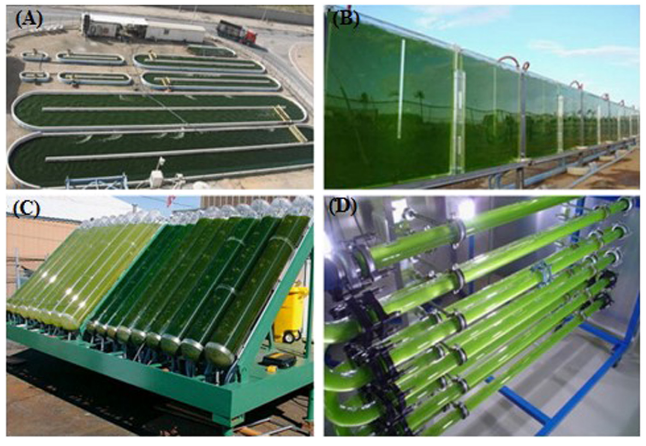
\includegraphics[width=0.7\linewidth]{LaTeX/raceways}
		\caption{Raceways and closed loop systems (Adeniyi et al., 2018)}
		\label{fig:raceways}
	\end{figure}
	


	As the algae grows and reproduces, carbon will accumulate in the system
	in the form of glucose, and within the oils that algae produce to store
	energy long term. The oils produced by certain species of algae contain
	high content of lipids; a portion of which are fatty acids. Fatty acids
	are long hydrocarbon chains with a carboxyl group at one end.
	Harvested biomass is processed, and oils are extracted. The dried
	biomass then undergoes pyrolysis, which converts any remaining compounds
	into bio-oil, and similar by-products to crude oil (U.S. Department of
	Agriculture, n.d.). 
	\newpage
	\textbf{Algae to biofuel synthesis}\\
	Processing of algal/bio-oils is less efficient than crude oils. Since
	the main source of hydrocarbon chains is fatty acids, the carboxyl group
	adds a significant amount of oxygen to the reaction mixture. While
	pyrolysis of crude oil is often aided by a catalyst, effective pyrolysis
	of bio oils requires one.
	
	\textit{Biogasoline production by co‐cracking of model compound mixture of bio‐oil and ethanol over HSZM‐5} (2014) by Wang et al.  investigated the effect of temperature, pressure, additives, and
	presence of a catalyst on the yield of high-grade hydrocarbon fuels. It
	was found that the addition of ethanol to the cracking mixture improved
	yields significantly. Ethanol improves the $H/C_\textrm{eff}$ (Hydrogen to carbon
	effective ratio) of reactants, which was previously found to improve
	cracking performance. Furthermore, the oxygen present in the hydroxyl
	group ($OH$) is likely to join with excess carbon to form $CO_x$ compounds and
	$H_2O$, as opposed to forming $CH_3COOH$ (acetic acid) or other
	by-products/coking agents. 
	\begin{figure}
	\centering
	
\includegraphics[width=0.15\paperwidth]{/home/noah/Documents/Obsidian/NoahsObsidianSync/NoahsObsidianSync/Images/Pasted image 20250813142529.png}\\
	\caption{Ethanol Structure}
	\end{figure}
	Ethanol
	
	At $400^\circ C,\; 2MPa$, $99\%$ and $91.5\%$ of the product was hydrocarbons
	and aromatic hydrocarbons by weight respectively. While coking did
	occur, use of the catalyst HSZM-5 improved yields, and was stable enough
	for coke removal to be achieved through combustion, allowing for reuse
	of catalyst. The high hydrocarbon content of the final product is
	commendable; however, this does not equate to a high yield. While the
	overall selectivity, or ratio of oil weight to final usable product
	weight, was $31.5\%$, this is lower than crude oil\textquotesingle s $43.3\%$ when it is cracked to form
	components of similar high-quality fuel at lab scale (Akah et al.,
	2025). 
	
	\subsubsection{Performance}\label{performance}

	\textbf{Exhaust gas temperature and
		power}\label{exhaust-gas-temperature-and-power}
	
	When complete combustion occurs, all hydrocarbon bonds are broken, and
	reformed into $CO_2$ and $H_2O$. This results in the maximum amount of energy
	being released. The conversion of liquid fuels into gasses, and the
	rapid release of energy as heat result in increased cylinder pressure,
	and therefore more \textquotesingle power\textquotesingle{} being
	generated by the engine. 
	
	While the output of an engine can be measured using a dynamo, this gives
	in incomplete picture of how much combustion is actually occurring. 
	Therefore exhaust gas temperature (EGT) is also measured. A higher
	exhaust gas temperature generally means that a larger portion of
	combustion is occurring with optimal stoichiometric ratios. When fuels
	have similar energy content, exhaust gas temperature can be directly
	compared to determine which fuel has more desirable combustion
	characteristics.\\
	(Ge et al., 2022)
	
	\textbf{Metrics}\label{metrics}\newline
	Ge et al. (2022) compared the performance of a cooking oil derived bio
	gasoline synthesised using similar cracking techniques. Studies on the
	combustion characteristics on algal derived fuels are sparse, but the
	bio oil the fuels are derived from both contain similar fatty acids, and
	once pyrolysed, their products are nearly identical in terms of
	hydrocarbon make up. 
	
\begin{figure}[h]
	\centering
		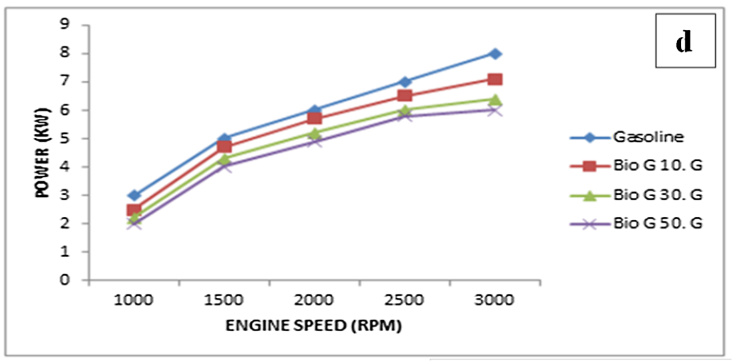
\includegraphics[width=0.5\paperwidth]{/home/noah/Documents/Obsidian/NoahsObsidianSync/NoahsObsidianSync/Images/Pasted image 20250813201748.png}\\
		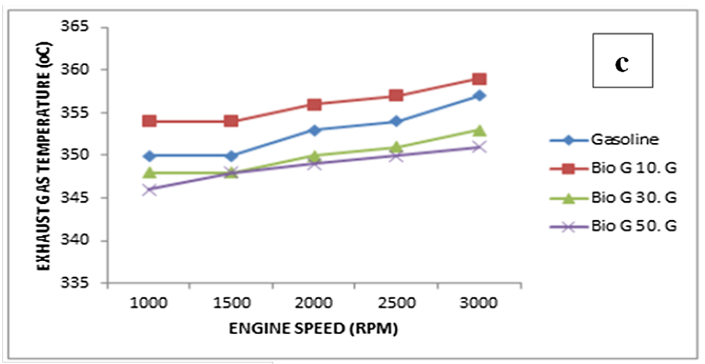
\includegraphics[width=0.5\paperwidth]{/home/noah/Documents/Obsidian/NoahsObsidianSync/NoahsObsidianSync/Images/Pasted image 20250813201757.png}\\
		\caption{Performance metrics over engine speed}
\end{figure}


	
	It was found that as biogasoline proportion of the fuel increased, both
	power, and EGT increased in a loosely quadratic manner. At lower
	concentrations, such as $10\%$, biogasoline exceeds the performance of
	regular gasoline alone, and demonstrates higher power, and EGT. This
	indicates that this blend combusts more completely, and offers superior
	performance to gasoline alone.\newpage
	
	\begin{figure}[h!]
		\centering
		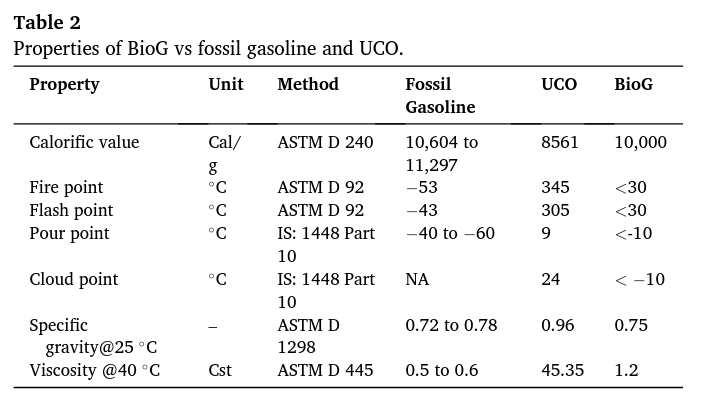
\includegraphics[width=0.5\paperwidth]{/home/noah/Documents/Obsidian/NoahsObsidianSync/NoahsObsidianSync/Images/Pasted image 20250708151954.png}\\
		\caption{Properties of Biogasoline and Fossil Gasoline}
	\end{figure}
	
	However, once the biogasoline concentration was increased to $30\%$, and
	beyond, decreases in power and EGT are apparent. The difference between
	the power generated by Bio G10. G and Bio G50. G was $2\ \mathrm{kW}$, roughly $19\%$ of the engines total rated capacity. Considering such a loss in performance, it must be questioned whether biogasoline is truly a 1:1 replacement as many sources suggest. 
	

	
	The caloric value of biogasoline was found to be only $94-89\%$ of
	unleaded gasoline 	(Ge et al., 2022), which somewhat accounts for the lower performance,
	however this is clearly not the only factor at play; As mentioned
	before, the $10\%$ blend performed better than gasoline alone. 
	
	\subsubsection{Tailpipe Emissions}\label{burning-emissions}
	
	A closely related topic is the fuel\textquotesingle s burning emissions.
	As mentioned previously, combustion characteristics differ between
	fuels. The amount of fuel being burnt daily is tremendous; Transitioning
	to a fuel with higher emissions will multiply even the smallest
	difference many times. Further considering the lower energy content of
	biogasoline, more fuel will be required to release the same amount of
	energy, therefore higher greenhouse gas (GHG) or nitric oxide ($NO_x$)
	emissions per gram will further contribute to the issue. 
	
	It should be mentioned that while the carbon released from combustion of
	biogasoline is derived from the atmosphere and therefore "net zero". 
	Tailpipe emissions of $CO_2$ aren\textquotesingle t necessarily a concern,
	however, $CO$ and $NO_x$ emissions require investigation, as both have much
	higher potential to harm people. $NO_x$ emissions in particular are
	exceedingly concerning, as they can form nitric acid rain, and are not
	reabsorbed during algae production. 
	
\begin{figure}[h]
	\centering
		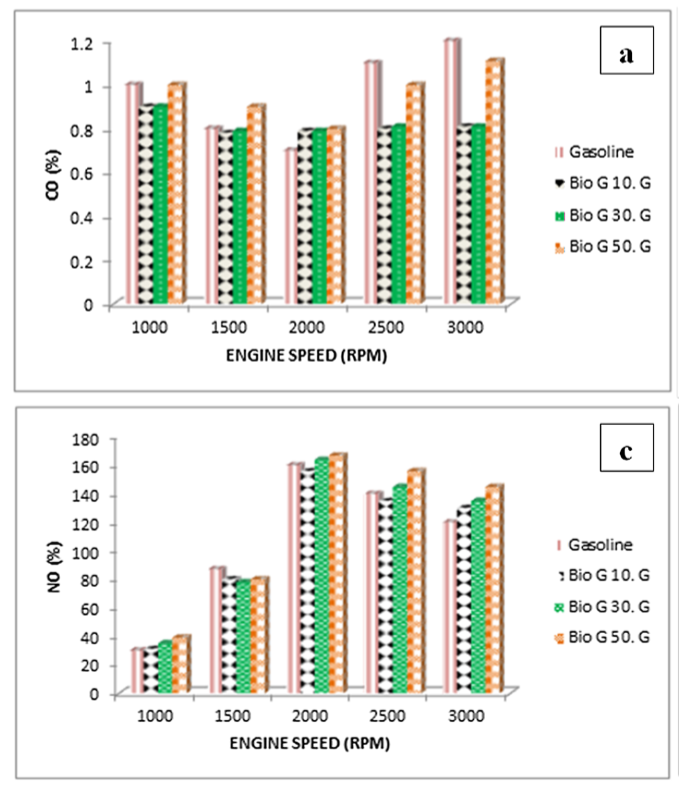
\includegraphics[width=0.4\paperwidth]{/home/noah/Documents/Obsidian/NoahsObsidianSync/NoahsObsidianSync/Images/Pasted image 20250814080904.png}\\
		\caption{Emissions over engine speed (Ge et al., 2022)}
		\label{EmissionsOverEngineSpeed}
\end{figure}

	
\begin{figure}[h]
	\centering
		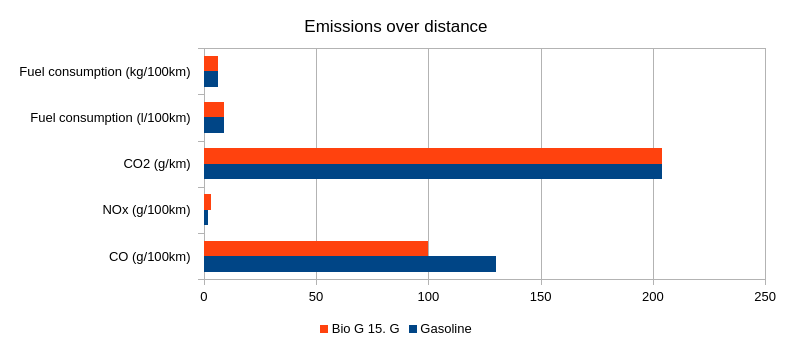
\includegraphics[width=0.6\paperwidth]{/home/noah/Documents/Obsidian/NoahsObsidianSync/NoahsObsidianSync/Images/Pasted image 20250814081941.png}\\
		\caption{Emissions over distance (Aakko-Saksa et al., 2011)}
		\label{EmissionsOverDistance}
\end{figure}

	
	Considering the previously cited study by Ge et al. (2022), and
	Aakko-Saksa et al. (2011), a clear trend can be observed.
	At low biogasoline concentrations by weight, $NO_x$ emissions are decreased, however once concentrations increase past $\approx 10\%$,	$NO_x$ emissions increase to match, or exceed under high load as shown in
	Figure 	\ref{EmissionsOverDistance}, the emissions of gasoline. It appears that large quantities of biogasoline as a fuel additive marginally increases $NO_x$ emissions, much like other \textquotesingle{}green\textquotesingle{} fuels such as \textquotesingle{} E10 \textquotesingle \cite{NSWGov_n.d.}.
	\subsection{Discussion}
	The synthesis of biogasoline is incredibly similar to that of gasoline. It can easily be inferred that with enough feedstock, biogasoline could be produced on scale with similar yields. While algal feedstock production is currently low, it's unique ability to be grown in aquatic environments allows opens up opportunities for large scale production; Not to mention the fact that it is a renewable resource, unlike conventional fossil fuels. 
	It appears that low concentrations of biogasoline produce more power than gasoline alone, attempting to run an engine on exclusive biogasoline may yield significant penalties and losses. While biogasoline does possess a lower caloric energy content, the difference is relatively small ($\approx 10\%$). In the future, it is possible that vehicles could be designed to be adapt to the combustion properties of biogasoline, much like they were for ethanol blends.\\
	Increased $NO_x$ emissions are somewhat concerning, with a 15\% blend demonstrating a 28.1\% increase (Figure \ref{EmissionsOverDistance}), however these were still below the Euro 5 limit. While significant GHG's are produced during synthesis, these and tailpipe emissions of $CO_2$, and $CO$ to some extent, are considered to be nullified by the fact that the carbon released was absorbed from the atmosphere, and therefore there is no real net increase in carbon abundance in the atmosphere.
	\subsubsection{Overall viability}
	
	\subsubsection{Limitations}\label{limitations} 

		\textbf{Lab Scale}\\
		The synthesis methods investigated were preformed on lab scale, and therefore do not fully represent the yields of industrial production.\\
		\textbf{Fuels derived from alternative feed stock investigated}\\
		As previously mentioned, the emissions figures provided by Ge et al. were based on fuel derived from used cooking oil. While the gasoline is very similar, the hydrocarbon's present are in different concentrations. The figures present likely do not accurate represent algal bio fuels, but the fuel general characteristics were considered similar enough, and multiple studies were considered when emissions were compared.

\subsubsection{Extensions}
\textbf{100\% biogasoline}\\
Studies that studies the characteristics of engines running on biogasoline alone were sparse, and often not accessible. This is concerning, as many consider biogasoline to be a 1:1 replacement for gasoline solely based on the presence of similar hydrocarbons. Investigation of the performance of pure biogasoline could reveal potential issues with it as a fuel source in the future. \\
\textbf{Comparison to other \textquotesingle{}green\textquotesingle{} fuels}\\
Ethanol fuels and fuel blends have been a topic of discussion for a significant period of time. Alternative processes allow algal biomass to be fermented due to its high glucose content. Further investigation of such synthesis processes could consider whether the advantages of algae as a feedstock could make it viable as a replacement for traditional stocks, like cane or sugar beet.
\textbf{Flexibility}\\
While not explicitly mentioned, algae speces can be grown in a variety of climates.
	\subsubsection{Conclusion}\label{conclusion} 
	Overall, biogasoline shows promise to be a competitive renewable fuel in future. It's production process is unique and offers many advantages to both biofuels 
	
	While its combustion properties differ from conventional gasoline, they are not necessarily worse. Biogasoline does have a lower energy content per gram ($\approx 10\%$), but passenger vesicles will likely not be hindered in their ability to operate based on this factor alone.
	
	Emissions data presents a mixed picture, but it seems that high concentration fuels may increase $NO_x$ emissions. Further investigation is required to determine the impact and potential mitigation techniques. 
	
	With investment and adoption, biogasoline possesses desirable properties and is a viable long term replacement for gasoline. 
	
	\newpage

	\bibliographystyle{apalike}
	\bibliography{Bibliography.bib}
	\nocite{*}
\end{document}